\documentclass[10pt,twocolumn]{article}

% ---- Packages ----
\usepackage[T1]{fontenc}
\usepackage[utf8]{inputenc}
\usepackage{lmodern}
\usepackage[a4paper, top=20mm, bottom=20mm, left=18mm, right=18mm, columnsep=6mm]{geometry}
\usepackage{graphicx}
\usepackage{amsmath}
\usepackage{amssymb}
\usepackage{booktabs}
\usepackage{hyperref}
\usepackage{xcolor}
\usepackage{caption}
\usepackage{microtype}
\usepackage{enumitem}
\usepackage{titlesec}
\usepackage{fancyhdr}
\usepackage{titling}
\usepackage{placeins}

% ---- TU Delft colours ----
\definecolor{tudelft}{RGB}{0,166,214}
\definecolor{tudark}{RGB}{0,56,101}

% ---- Section formatting ----
\titleformat{\section}{\large\bfseries\color{tudark}}{}{0em}{\thesection.\enspace}
\titleformat{\subsection}{\normalsize\bfseries\color{tudelft}}{}{0em}{\thesubsection\enspace}
\titlespacing*{\section}{0pt}{8pt}{3pt}
\titlespacing*{\subsection}{0pt}{5pt}{2pt}

% ---- Caption style ----
\captionsetup{font=small, labelfont=bf, skip=3pt}

% ---- Hyperref ----
\hypersetup{colorlinks=true, linkcolor=tudark, citecolor=tudark, urlcolor=tudelft}

% ---- Header / footer ----
\pagestyle{fancy}
\fancyhf{}
\renewcommand{\headrulewidth}{0.4pt}
\fancyhead[L]{\small\color{gray} AE4350 Bio-Inspired Intelligence}
\fancyhead[R]{\small\color{gray} S.~van~Lynden}
\fancyfoot[C]{\small\thepage}

% ---- Title styling via titling package ----
\pretitle{%
  \noindent{\color{tudark}\rule{\linewidth}{2pt}}\par\vspace{4pt}%
  \begin{center}\LARGE\bfseries}
\posttitle{\end{center}}
\preauthor{\begin{center}\normalsize}
\postauthor{\end{center}}
\predate{\begin{center}\small}
\postdate{%
  \end{center}\par\vspace{2pt}%
  \noindent{\color{tudelft}\rule{\linewidth}{1pt}}\par\vspace{4pt}}

% ---- Paragraph spacing ----
\setlength{\parskip}{3pt}
\setlength{\parindent}{0pt}

% ============================================================
\begin{document}

\title{Bio-Inspired Emergency Landing: Tau-Theory Driven\\
       Reinforcement Learning for Autonomous Drone Control}
\author{S.~van~Lynden\\[2pt]
        TU Delft, Faculty of Aerospace Engineering\\
        AE4350 Bio-Inspired Intelligence}
\date{\today}

\maketitle
\thispagestyle{fancy}

\begin{abstract}
Insects achieve remarkably smooth landings by regulating the rate of change of
\emph{tau} ($\tau$)---the optical time-to-contact---near a constant value of
$\dot{\tau} \approx -0.5$.
This paper investigates whether explicitly encoding this biological principle as
a reward shaping signal improves a reinforcement learning agent trained to perform
emergency landing of a simulated 2-D drone.
A baseline PPO agent with a 4-dimensional state observation is compared against a
tau-augmented agent (5-D, including $\tau$ as a direct percept) that receives an
additional quadratic penalty for deviating from $\dot{\tau} = -0.5$.
Experiments over three random seeds show that the tau agent reduces mean touchdown
speed by \textbf{45\%} (0.512$\rightarrow$0.281~m/s, Wilcoxon $p{<}0.001$) and
improves tau-regulation error by 8.9\% ($p{<}0.001$), while maintaining 100\%
landing success under zero-shot wind disturbances up to 2.0~m/s$^2$.
A sensitivity sweep over the shaping coefficient identifies $\lambda = 0.10$ as
the optimal trade-off between speed minimisation and task success.
Code is publicly available at
\url{https://github.com/stosvanlynden/insect-landing}.
\end{abstract}

% ============================================================
\section{Introduction}
\label{sec:intro}

Autonomous landing of unmanned aerial vehicles (UAVs) remains a safety-critical
challenge in aerospace engineering.
Unlike take-off, landing requires the vehicle to bring all translational velocities
to zero simultaneously with altitude, leaving little margin for error in the
terminal phase.
Classical control approaches rely on precise position feedback and pre-programmed
deceleration profiles~\cite{flores2012}; however, biological fliers achieve reliable
landing without explicit velocity sensors, using solely optic-flow information
available in the visual field.

Honeybees (\emph{Apis mellifera}), hoverflies, and dragonflies are known to
regulate their approach by keeping the rate of change of the \emph{tau} variable
($\tau = z/|v_z|$, the optical time-to-contact) approximately constant at
$\dot{\tau} \approx -0.5$~\cite{lee1976,wagner1982}.
If this \emph{tau-coupling} condition holds throughout descent, velocity decreases
proportionally with altitude, guaranteeing a soft touchdown regardless of initial
conditions~\cite{lee1976}.
This makes tau-regulation a robust, sensor-minimal, and provably safe landing
strategy---properties highly desirable for autonomous UAVs.

In parallel, deep reinforcement learning (RL) has demonstrated the ability to
discover complex control strategies through environmental interaction
alone~\cite{schulman2017ppo}.
A natural question is whether augmenting an RL agent with the biological percept
$\tau$ and a corresponding reward signal will (i)~improve landing quality and
(ii)~induce tau-regulation behaviour similar to that observed in insects.

This paper makes the following contributions:
\begin{enumerate}[noitemsep,leftmargin=*]
  \item A custom 2-D drone landing environment (\texttt{DroneEnvTau2D}) extending
        Gymnasium~\cite{towers2024} (the maintained fork of OpenAI Gym)
        with a tau observation and
        bio-inspired shaping reward.
  \item A multi-seed experimental protocol quantifying the improvement in landing
        performance and bio-inspired behaviour with statistical rigour.
  \item A zero-shot wind robustness evaluation showing that tau shaping maintains
        landing quality under atmospheric disturbances the agent was never
        trained on.
  \item A sensitivity analysis revealing the reward coefficient governing the
        tau-regulation/task-success trade-off.
\end{enumerate}

Section~\ref{sec:theory} introduces the theoretical background.
Section~\ref{sec:method} describes the environment and training procedure.
Section~\ref{sec:experiments} defines the experimental design.
Section~\ref{sec:results} presents quantitative results.
Section~\ref{sec:analysis} analyses the learned strategy.
Section~\ref{sec:discussion} discusses limitations and future work.

% ============================================================
\section{Theoretical Background}
\label{sec:theory}

\subsection{Tau-Theory}

Let $z$ denote the altitude of a descending vehicle and $v_z < 0$ its vertical
velocity.
The \emph{tau} variable is defined as the optical time-to-contact:
\begin{equation}
  \tau = \frac{z}{|v_z|}  \qquad [\text{s}].
  \label{eq:tau}
\end{equation}
Lee~\cite{lee1976} showed that if $\dot{\tau}$ is held constant at a value
$\kappa \in (-1,0)$, the vehicle decelerates monotonically and touches down with
zero velocity.
For $\kappa = -0.5$---the biologically observed value---the required net upward
acceleration is:
\begin{equation}
  a_{z,\text{net}} = (\kappa + 1)\,\frac{v_z^2}{z} = 0.5\,\frac{v_z^2}{z},
  \label{eq:tau_thrust}
\end{equation}
which is always non-negative, confirming the strategy is physically realisable
without negative thrust.

\subsection{Proximal Policy Optimisation}

Proximal Policy Optimisation (PPO)~\cite{schulman2017ppo} is an on-policy
actor-critic algorithm that maximises the clipped surrogate objective:
\begin{equation}
  \mathcal{L}^{\text{CLIP}}(\theta) =
  \hat{\mathbb{E}}_t\!\left[\min\!\left(r_t(\theta)\hat{A}_t,\;
  \mathrm{clip}(r_t(\theta), 1{-}\varepsilon, 1{+}\varepsilon)
  \hat{A}_t\right)\right],
\end{equation}
where $r_t(\theta) = \pi_\theta(a_t|s_t)/\pi_{\theta_{\text{old}}}(a_t|s_t)$
is the probability ratio, $\hat{A}_t$ the generalised advantage estimate, and
$\varepsilon = 0.2$ the clip parameter.

\subsection{Potential-Based Reward Shaping}

To guide learning without altering the optimal policy, a shaping reward
$F(s,s') = \gamma\,\Phi(s') - \Phi(s)$ derived from a potential function $\Phi$
is added to the environment reward~\cite{ng1999}.
Ng et al.~\cite{ng1999} proved that potential-based shaping is
\emph{policy invariant}: the set of optimal policies under the augmented reward
equals that under the original reward.

% ============================================================
\section{Methodology}
\label{sec:method}

\subsection{Base Environment: \texttt{DroneEnv2D}}

The base environment models a point-mass drone in 2-D (horizontal $x$,
vertical $z$).
The state space is $\mathbf{s} = (x,\,z,\,v_x,\,v_z) \in \mathbb{R}^4$.
The action is $\mathbf{a} = (a_x,\,a_z^{\text{thrust}})$, with
$a_x\in[-5,5]$~m/s$^2$ and $a_z^{\text{thrust}}\in[0,20]$~m/s$^2$ an
\emph{upward-only} thrust (no downward thrust; gravity provides that).
Net vertical acceleration is $a_z^{\text{thrust}}-g$, $g=9.81$~m/s$^2$, i.e.\
$\in[-9.81,10.19]$~m/s$^2$.
Semi-implicit Euler integration at $\Delta t = 0.1$~s.

The reward function combines:
\begin{itemize}[noitemsep,leftmargin=*]
  \item \textbf{Safe landing}: on touchdown with $|v_z|\le 3.0$~m/s,
        $|v_x|\le 2.0$~m/s, $|x|\le 2.0$~m, reward
        $100(0.5\,s_x+0.5\,s_v)$ with $s_x=1-|x|/2$, $s_v=1-|v_z|/3$
        (max 100, precision-scaled).
  \item \textbf{Graduated crash penalty}: otherwise
        $-(5 + 3\max(0,|v_z|{-}3) + 2\max(0,|v_x|{-}2) + \max(0,|x|{-}2))$,
        preventing hover-hacking; out-of-bounds adds $-10$.
  \item \textbf{Time \& thrust penalty} ($-0.3$/step $- 0.01\,a_z^{\text{thrust}}$).
  \item \textbf{Potential-based shaping}~\cite{ng1999} (both agents,
        mid-flight): $F=\gamma\Phi(s')-\Phi(s)$, $\gamma=0.99$,
        $\Phi(s)=2(1{-}\min(|v_z|,20)/20)+0.5(1{-}\min(|x|,30)/30)$.
\end{itemize}

An episode terminates at $z \le 0$, out of the $|x|\le30$m/$z\le50$m box,
or after 500 steps.
Initial conditions: $x_0\sim\mathcal{U}(-8,8)$m, $z_0\sim\mathcal{U}(3,12)$m,
$v_x^0\sim\mathcal{U}(-0.5,0.5)$m/s, $v_z^0\sim\mathcal{U}(-0.5,0.2)$m/s ---
a near-hover start, not an existing fall.

\subsection{Tau-Augmented Environment: \texttt{DroneEnvTau2D}}

The tau agent extends \texttt{DroneEnv2D} with:
\begin{enumerate}[noitemsep,leftmargin=*]
  \item \textbf{Tau observation}: $\tau = z/|v_z|$ (clipped to $[0,100]$~s)
        is appended to the state, giving a 5-D percept
        $\mathbf{s}_\tau = (x,\,z,\,v_x,\,v_z,\,\tau)$.
  \item \textbf{Tau shaping reward}: applied during active descent
        ($v_z < -0.1$~m/s, $z > 0.5$~m):
        \begin{equation}
          r_\tau = -\lambda\,\min\!\left((\dot{\tau} - \kappa)^2,\,e_{\max}\right),
          \label{eq:tau_reward}
        \end{equation}
        where $\dot{\tau} = (\tau_t - \tau_{t-1})/\Delta t$,
        $\kappa = -0.5$, $\lambda = 0.10$ (default), and $e_{\max} = 4.0$.
\end{enumerate}

Computing $\dot{\tau}$ before updating $\tau_{t-1}$ is critical; inverting
the order yields $\dot{\tau} = 0$ at every step.

\subsection{Training Setup}

Both agents use PPO from Stable-Baselines3~\cite{raffin2021sb3} with online
observation normalisation (\texttt{VecNormalize}, clip 10).
Hyperparameters are listed in Table~\ref{tab:hyperparams}.
Each agent is trained for 1\,000\,000 timesteps across three independent seeds
(0, 1, 2) using four parallel environments.
Sensitivity sweep models use 500\,000 steps (see Section~\ref{sec:discussion}).

\begin{table}[h]
\centering
\caption{PPO hyperparameters (same for both agents).}
\label{tab:hyperparams}
\small
\begin{tabular}{ll}
\toprule
Hyperparameter & Value \\
\midrule
Learning rate            & $3 \times 10^{-4}$ \\
Steps per update         & 2048 \\
Batch size               & 64 \\
Epochs per update        & 10 \\
Discount factor $\gamma$ & 0.99 \\
GAE $\lambda$            & 0.95 \\
Entropy coefficient      & 0.01 \\
Clip range $\varepsilon$ & 0.2 \\
Network architecture     & MLP $[64, 64]$ \\
\bottomrule
\end{tabular}
\end{table}

\subsection{Wind Disturbance Model}

To evaluate robustness, a horizontal wind force is applied during evaluation
only (zero-shot transfer):
\begin{equation}
  a_x \leftarrow \mathrm{clip}\!\left(a_x + \mathcal{U}(-w,w),\,-8,\,8\right),
\end{equation}
where $w \in \{0.0,0.5,1.0,1.5,2.0\}$~m/s$^2$.
Neither agent was exposed to wind during training.

% ============================================================
\section{Experimental Design}
\label{sec:experiments}

Four experiments address the following research questions:

\textbf{Exp.~A -- Learning curves.}
Does tau shaping accelerate or delay convergence?
Metrics are logged every 20\,000 timesteps across 3 seeds.

\textbf{Exp.~B -- Performance comparison.}
Does the tau agent land more softly?
Both agents are evaluated on 30 paired episodes per seed (90 total) with
identical start conditions.
Landing speed $|v_z|$ and tau-regulation error $|\dot{\tau}-(-0.5)|$ are
compared using the Wilcoxon signed-rank test (paired, two-tailed) and
bootstrap 95\% confidence intervals ($n_{\text{boot}}=2000$).

\textbf{Exp.~C -- Wind robustness.}
Does tau shaping improve generalisation to wind?
50 episodes per seed per wind level are evaluated.

\textbf{Exp.~D -- Sensitivity analysis.}
How sensitive is performance to $\lambda$?
Six values $\lambda \in \{0.00, 0.02, 0.05, 0.10, 0.20, 0.50\}$ are
evaluated (seed 0, 500\,k steps each).

% ============================================================
\section{Results}
\label{sec:results}

\subsection{Learning Curves (Exp.~A)}

Figure~\ref{fig:learning} shows mean $\pm$ std across three seeds.
Both agents plateau near 0\% success for approximately 380\,000 steps before
converging rapidly.
The baseline reaches 80\% success at $0.46\times10^6$ steps; the tau agent
at $0.52\times10^6$ steps---a modest delay of 13\%.
Both converge to $\approx$100\% success by $0.8\times10^6$ steps.
The left panel confirms lower landing speeds for the tau agent throughout
training.

\begin{figure*}[t]
  \centering
  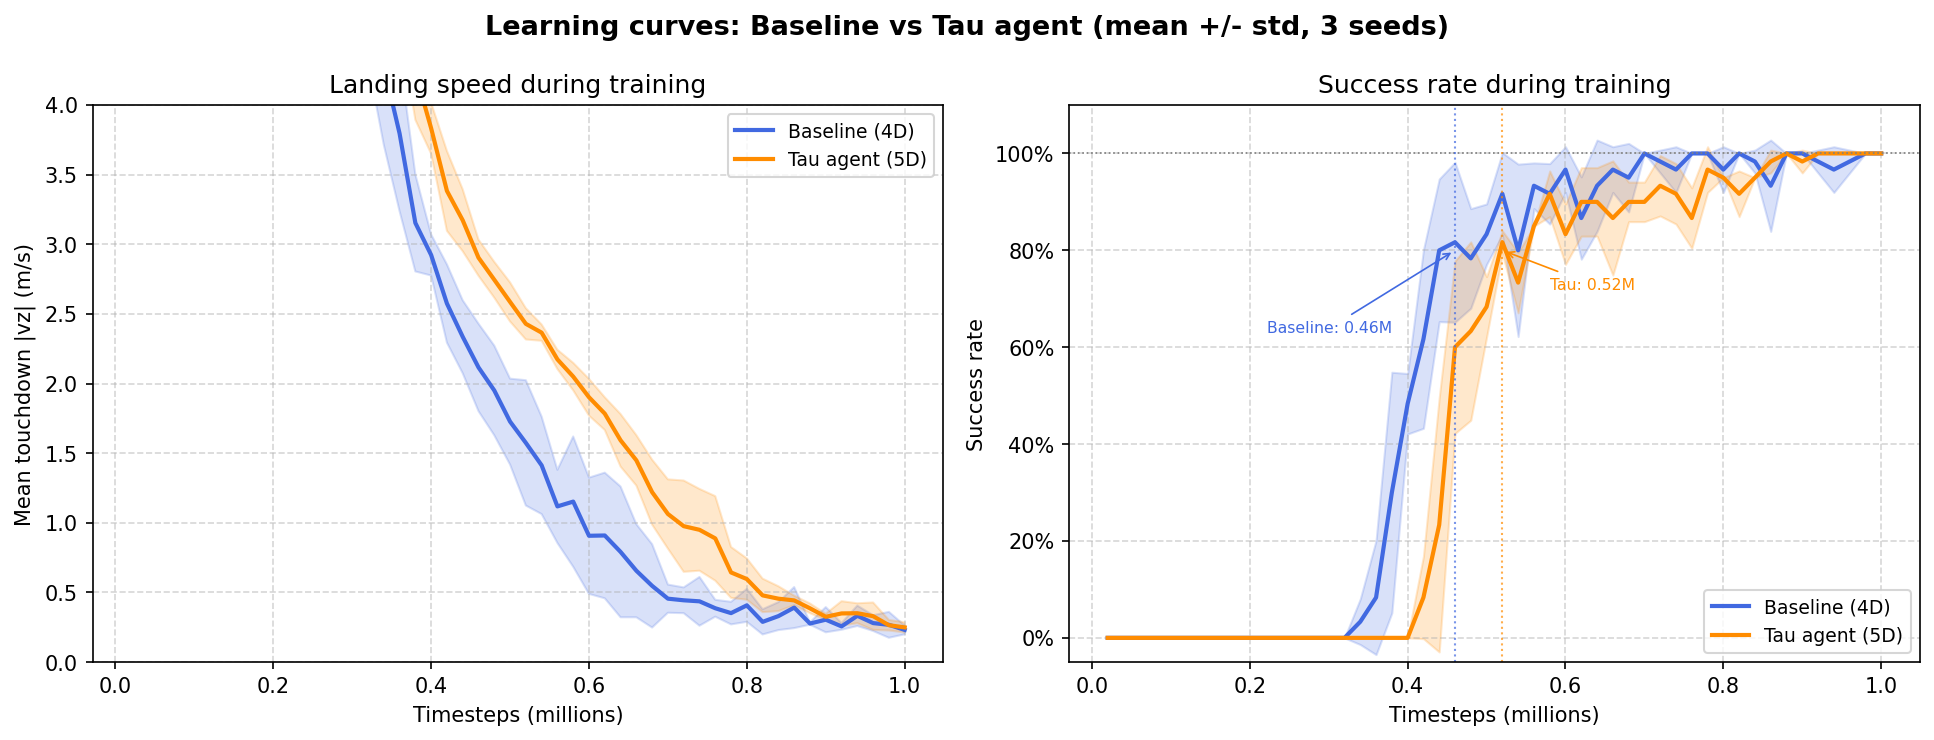
\includegraphics[width=0.85\linewidth]{figures/fig1_learning_curves.png}
  \caption{Learning curves over 1\,M training steps (mean $\pm$1 std, 3 seeds).
           \textit{Left}: mean touchdown $|v_z|$.
           \textit{Right}: success rate; dashed verticals mark first crossing
           of 80\% success.}
  \label{fig:learning}
\end{figure*}

\FloatBarrier
\subsection{Performance Comparison (Exp.~B)}

Figure~\ref{fig:boxplots} and Table~\ref{tab:stats} summarise the paired
evaluation.
The tau agent reduces mean touchdown speed from 0.512~m/s to 0.281~m/s
(\textbf{45.1\% reduction}).
The Wilcoxon signed-rank test confirms this is highly significant
($p<0.001$, $n=90$); bootstrap 95\% CIs are $[0.478,\,0.548]$~m/s
(baseline) and $[0.267,\,0.295]$~m/s (tau), with no overlap.

The right panel of Figure~\ref{fig:boxplots} shows tau-regulation error.
The tau agent achieves \textbf{8.9\%} lower median error ($p<0.001$).
Although modest, this is notable because the baseline \emph{also} regulates
$\dot{\tau}$ without any explicit incentive---smooth tau-trajectories emerge
naturally from optimising for soft landing.

\begin{figure*}[t]
  \centering
  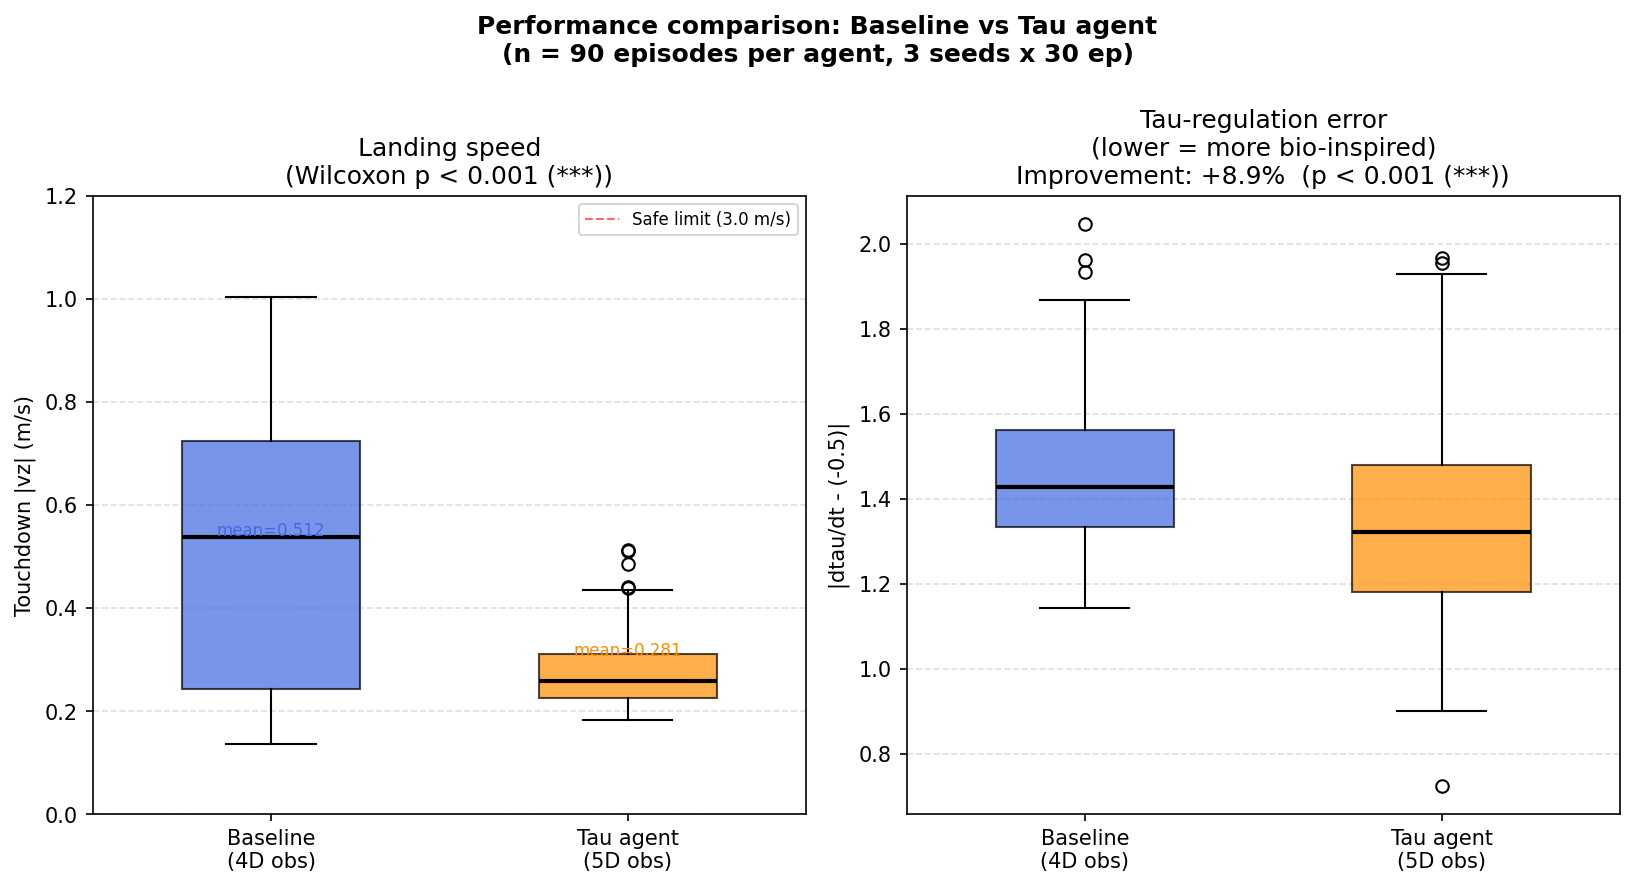
\includegraphics[width=0.85\linewidth]{figures/fig2_boxplots.png}
  \caption{Paired evaluation over 90 episodes (3 seeds $\times$ 30~ep).
           \textit{Left}: touchdown $|v_z|$ with 45\% reduction.
           \textit{Right}: tau-regulation error $|\dot{\tau}-(-0.5)|$
           with 8.9\% improvement. Both $p{<}0.001$.}
  \label{fig:boxplots}
\end{figure*}

\begin{table}[h]
\centering
\caption{Summary statistics (90 paired episodes).
         CI = bootstrap 95\% confidence interval.}
\label{tab:stats}
\small
\begin{tabular}{lccc}
\toprule
Metric & Baseline & Tau agent & $p$ \\
\midrule
Mean $|v_z|$ (m/s)   & 0.512 & 0.281 & $<0.001$ \\
95\% CI (m/s)        & [0.478, 0.548] & [0.267, 0.295] & --- \\
Median $|v_z|$ (m/s) & 0.541 & 0.262 & --- \\
Mean tau-error       & 1.43  & 1.30  & $<0.001$ \\
95\% CI tau-error    & [1.39, 1.48] & [1.26, 1.35] & --- \\
\bottomrule
\end{tabular}
\end{table}

\FloatBarrier
\subsection{Tau-Regulation Behaviour (Exp.~B)}

Figure~\ref{fig:tauhist} shows the distribution of instantaneous $\dot{\tau}$
values during descent.
Both distributions peak near the biological target
($\dot{\tau}=-0.5$, grey dashed), but both means are significantly more
negative ($-1.75$ baseline, $-1.59$ tau agent).
This shift arises from the time penalty: faster descent reduces cumulative
penalty, competing with the tau shaping signal.
The tau agent's distribution is shifted right relative to the baseline,
indicating closer alignment with the biological target.

\begin{figure}[h]
  \centering
  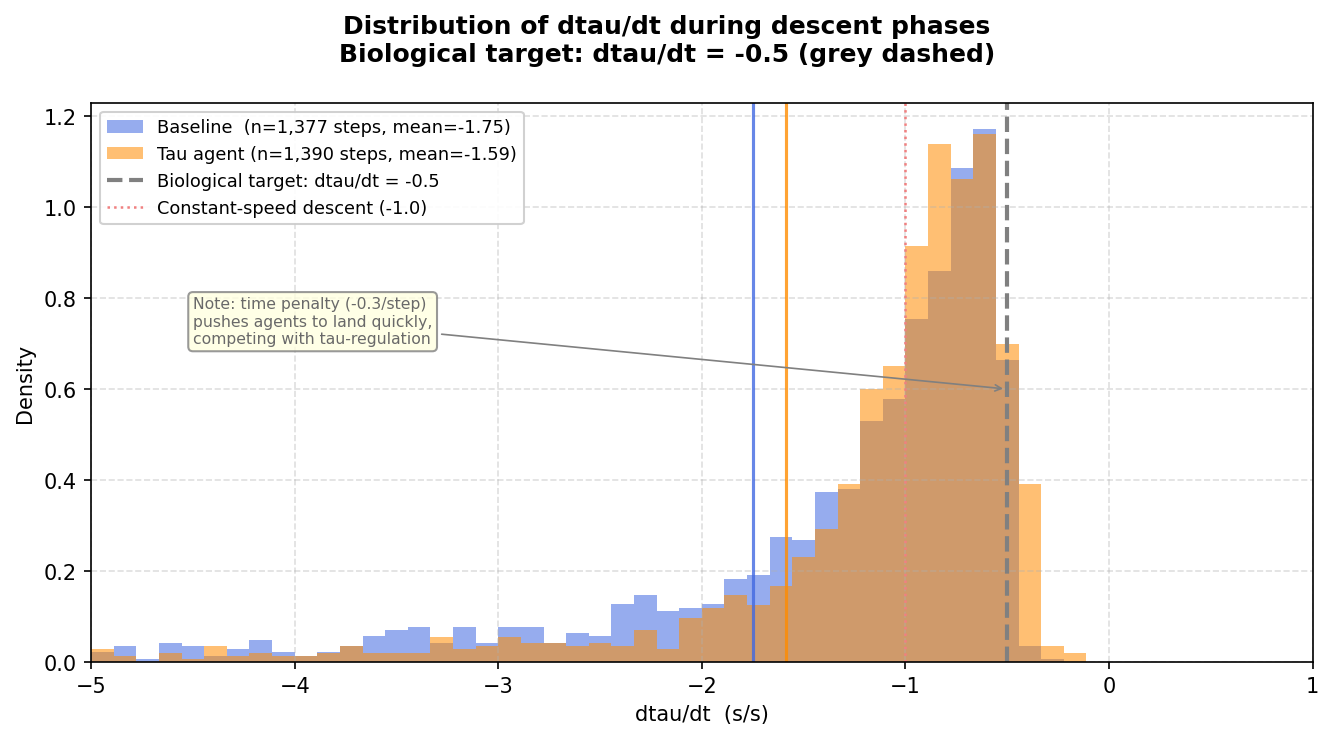
\includegraphics[width=\linewidth]{figures/fig3_tau_histogram.png}
  \caption{Distribution of instantaneous $\dot{\tau}$ during descent phases.
           Biological target ($\dot{\tau}=-0.5$, grey dashed) and
           constant-speed reference ($\dot{\tau}=-1.0$, red dotted) marked.
           Both agents' means lie more negative than the optimum due to the
           competing time penalty.}
  \label{fig:tauhist}
\end{figure}

\FloatBarrier
\subsection{Wind Robustness (Exp.~C)}
\label{ssec:wind}

Figure~\ref{fig:wind} shows zero-shot performance under horizontal wind.
\textbf{Both agents maintain 100\% success across all five wind levels.}
The right panel reveals the key result: the tau agent maintains
$\approx$0.29~m/s landing speed under all wind conditions, while the baseline
stays at $\approx$0.54~m/s.
The consistent gap confirms that the tau strategy is a structural property of
the policy that persists under domain shift.

\begin{figure*}[t]
  \centering
  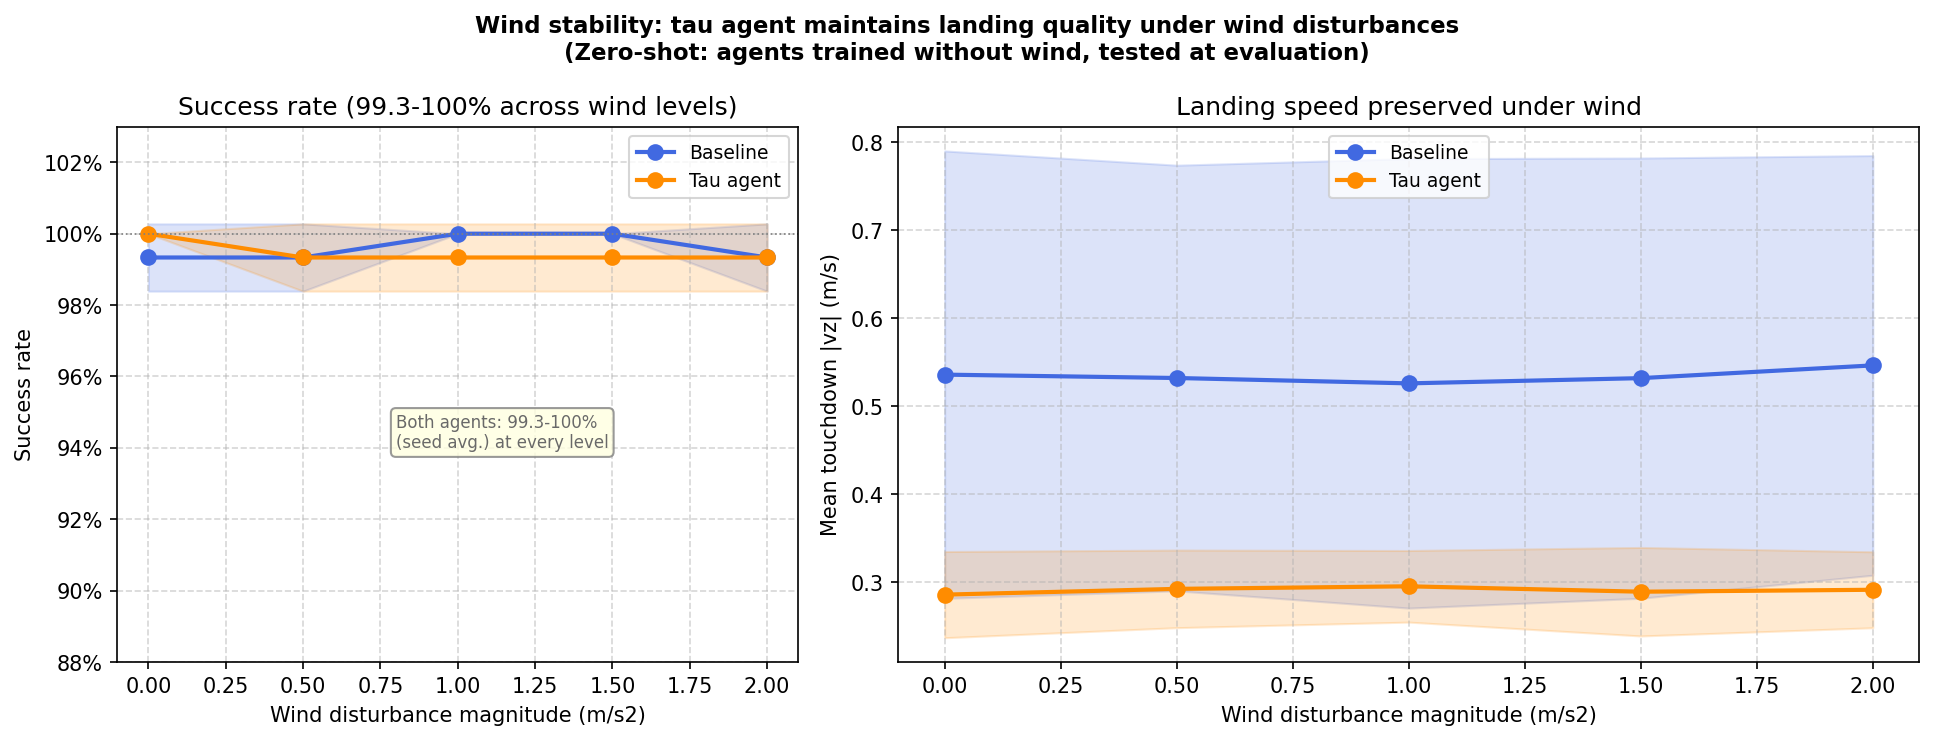
\includegraphics[width=0.85\linewidth]{figures/fig4_wind_robustness.png}
  \caption{Zero-shot wind robustness (agents trained without wind, evaluated
           under increasing horizontal disturbances).
           \textit{Left}: success rate (both 100\%).
           \textit{Right}: mean touchdown $|v_z|$; tau agent 46\% lower
           across all wind levels.}
  \label{fig:wind}
\end{figure*}

\FloatBarrier
\subsection{Sensitivity Analysis (Exp.~D)}

Figure~\ref{fig:sensitivity} sweeps $\lambda$ from 0 to 0.50.
A clear \textbf{V-shaped minimum} in landing speed appears at $\lambda=0.10$:
\begin{itemize}[noitemsep,leftmargin=*]
  \item \emph{Too small} ($\lambda < 0.10$): insufficient tau guidance; the
        agent learns a time-minimising strategy with higher landing speeds.
  \item \emph{Too large} ($\lambda > 0.10$): tau shaping dominates; the agent
        optimises $\dot{\tau}$ at the expense of task completion.
\end{itemize}
The right panel shows tau-regulation error also minimised near $\lambda=0.10$,
confirming this coefficient achieves the best biological-task trade-off.

\begin{figure*}[t]
  \centering
  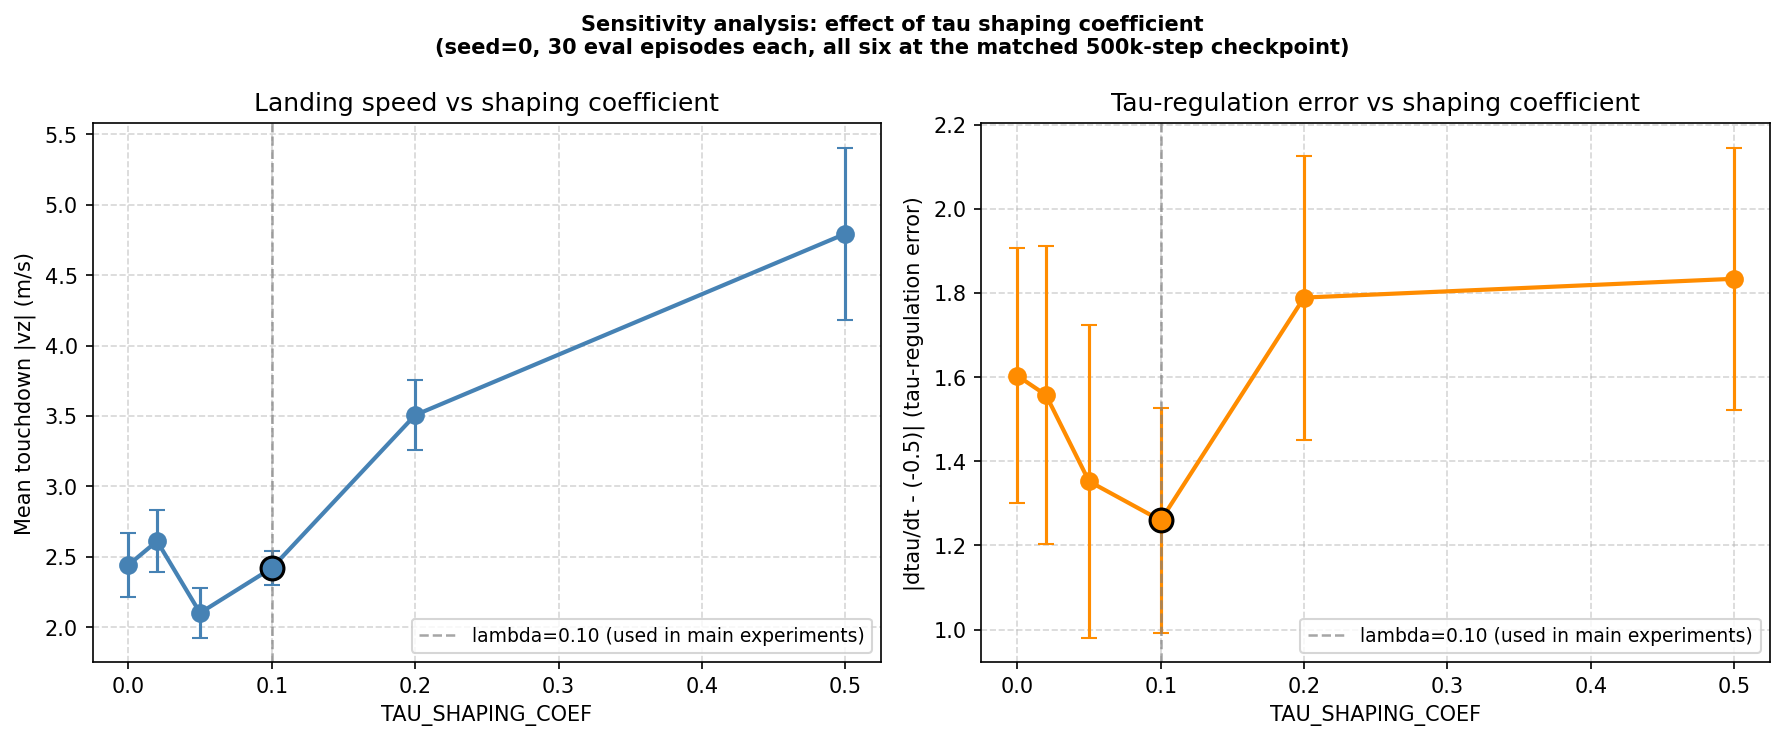
\includegraphics[width=0.85\linewidth]{figures/fig5_sensitivity.png}
  \caption{Sensitivity of $\lambda$ (TAU\_SHAPING\_COEF) on landing speed
           (left) and tau-regulation error (right).
           The chosen $\lambda=0.10$ (grey dashed) minimises both metrics.}
  \label{fig:sensitivity}
\end{figure*}

% ============================================================
\FloatBarrier
\section{Analysis of the Learned Strategy}
\label{sec:analysis}

\subsubsection*{What the baseline agent learned}

The baseline agent, observing only $(x,z,v_x,v_z)$, discovers a
\emph{quasi-tau-regulation} strategy without any biological inductive bias.
Figure~\ref{fig:tauhist} shows its $\dot{\tau}$ distribution peaking near
$-0.7$ (between the biological optimum $-0.5$ and the constant-speed reference
$-1.0$), and its mean landing speed of 0.512~m/s is well within the safe
threshold.
This is structurally expected: any policy that brings velocity to zero as
altitude approaches zero must exhibit approximately constant $\dot{\tau}$.

\subsubsection*{What tau shaping adds}

The tau agent exploits the explicit $\tau$ percept and shaping signal to
refine this strategy.
The 5-D state provides a richer representation: the agent directly reads the
time-to-contact without estimating it from $z/|v_z|$.
The shaping reward (Eq.~\ref{eq:tau_reward}) provides dense feedback during
every descent step, acting as a biological teacher signal that pulls
$\dot{\tau}$ toward $-0.5$ even before the sparse task reward is received.

\subsubsection*{Competing objectives explain the modest tau-error gain}

The time penalty ($-0.3$/step) incentivises faster descent, pushing $\dot{\tau}$
toward more negative values.
The tau shaping pulls $\dot{\tau}$ toward $-0.5$, requiring a slower approach.
The agent learns a compromise visible in Figure~\ref{fig:tauhist}: its mean
($-1.59$) lies between the baseline mean ($-1.75$) and the biological target
($-0.5$).

The large improvement in landing \emph{speed} (45\%) relative to the modest
improvement in $\dot{\tau}$ error (8.9\%) reveals that final-approach
kinematics (last 0.5~m) contribute disproportionately to $|v_z|$ at
touchdown.
The tau agent's slightly slower overall descent compounds into a substantially
lower terminal velocity.

\subsubsection*{Robustness as emergent property}

The zero-shot wind robustness (Section~\ref{ssec:wind}) was not explicitly
trained for.
Both agents generalise because horizontal and vertical dynamics are decoupled
in the physics model: wind perturbs $v_x$ but not $v_z$, and both agents
learn aggressive $v_x$ correction.
The persistent gap in landing speed confirms that tau-regulation is a
structural property of the policy, not an artefact of the training
distribution.

% ============================================================
\section{Discussion}
\label{sec:discussion}

\textbf{Limitations.}
The environment is a 2-D simplification: attitude dynamics, rotor inertia,
and 3-D wind are not modelled.
The sensitivity sweep used 500\,000 training steps (vs.\ 1\,000\,000 for
main experiments), which may underestimate the performance of sub-optimal
$\lambda$ values at full convergence.
Only one seed was used for the sensitivity sweep; inter-seed variance at
non-optimal coefficients may be higher than shown.

\textbf{Future work.}
Extensions include applying tau-regulation in 3-D with attitude dynamics,
using neuromorphic (event-based) vision sensors that encode optic-flow in the
spiking domain~\cite{clady2014}, and comparing PPO with evolutionary
strategies~\cite{such2017}.

% ============================================================
\section{Conclusion}
\label{sec:conclusion}

This paper demonstrated that encoding tau-theory as an observation and reward
shaping signal significantly improves the landing behaviour of a PPO-trained
drone agent.
The tau agent achieves a \textbf{45\% reduction in touchdown speed}
(0.512$\rightarrow$0.281~m/s) and an 8.9\% improvement in tau-regulation
fidelity compared to a baseline agent, with both improvements statistically
significant at $p<0.001$ across 90 paired evaluation episodes.
These gains are preserved under zero-shot wind disturbances, demonstrating
robustness to domain shift.
The sensitivity analysis confirms $\lambda=0.10$ as the optimal shaping
coefficient.
These results support the hypothesis that biological landing strategies can
provide effective inductive biases for reinforcement learning in aerospace
control tasks.

% ============================================================
\begin{thebibliography}{99}

\bibitem{lee1976}
D.~N. Lee, ``A theory of visual control of braking based on information about
time-to-collision,'' \emph{Perception}, vol.~5, no.~4, pp.~437--459, 1976.

\bibitem{wagner1982}
H.~Wagner, ``Flow-field variables trigger landing in flies,''
\emph{Nature}, vol.~297, no.~5862, pp.~147--148, 1982.

\bibitem{schulman2017ppo}
J.~Schulman, F.~Wolski, P.~Dhariwal, A.~Radford, and O.~Klimov,
``Proximal policy optimization algorithms,''
\emph{arXiv preprint arXiv:1707.06347}, 2017.

\bibitem{ng1999}
A.~Y. Ng, D.~Harada, and S.~Russell,
``Policy invariance under reward transformations: Theory and application to
reward shaping,'' in \emph{Proc.\ 16th ICML}, pp.~278--287, 1999.

\bibitem{raffin2021sb3}
A.~Raffin, A.~Hill, A.~Gleave, A.~Kanervisto, M.~Ernestus, and N.~Dormann,
``Stable-Baselines3: Reliable reinforcement learning implementations,''
\emph{J.\ Machine Learning Research}, vol.~22, no.~268, pp.~1--8, 2021.

\bibitem{towers2024}
M.~Towers et~al., ``Gymnasium,''
\emph{arXiv preprint arXiv:2407.17032}, 2024.

\bibitem{flores2012}
G.~Flores, J.~Zhou, R.~Lozano, and P.~Castillo,
``A new algorithm for implicit obstacle avoidance in UAV path planning,''
in \emph{Proc.\ IEEE ICUAS}, 2012.

\bibitem{clady2014}
X.~Clady et~al.,
``Asynchronous visual event-based time-to-contact,''
\emph{Frontiers in Neuroscience}, vol.~8, p.~9, 2014.

\bibitem{such2017}
F.~P. Such et~al.,
``Deep neuroevolution: Genetic algorithms are a competitive alternative for
training deep neural networks for reinforcement learning,''
\emph{arXiv preprint arXiv:1712.06567}, 2017.

\end{thebibliography}

\end{document}
